\section{Last but not least}
And finally we tackle generating our tree. I could only think of two ways of traversing the tree: (a) the lazy way and (b) the smart way.


\subsection{The lazy way}
The lazy way involves taking the two smallest (i.e. lowest occurring) characters from our map. We can then create a tuple with a value that is the sum of their corresponding value. This leaves us with a tuple that looks like
\begin{equation*}
    \texttt{\{:leaf, v1 + v2, \{:node, k1\}, \{:node, k2\}\}}
\end{equation*}

And then we continue by taking the next smallest character from our map and add its value to the value of the tuple we just created.
\begin{equation*}
    \texttt{
        \{:leaf, v3 + v1 + v2, \{:node, k3\},
        \{:leaf, v1 + v2, \{:node, k1\}, \{:node, k2\}\}
        \}
    }
\end{equation*}
We can continue this process until we have accounted for all the characters in our list. 
\pagebreak
\begin{lstlisting}[language=Elixir, title=The lazy way]
defmodule Lazy do
  def tree_start(map) do
    {kv1, map} = Mapper.min_pop(map)
    tree(kv1, map)
  end
  def tree({k1, v1}, map) do
    {{k2, v2}, map} = Mapper.min_pop(map)
    new_leaf = {:leaf, v1 + v2, {:node, k1}, {:node, k2}}
    tree(new_leaf, map)
  end
  def tree(tree, map) when map == %{} do
    tree
  end
  def tree({:leaf, v, l, r}, map) do
    {{k2, v2}, map} = Mapper.min_pop(map)
    new_leaf = {:leaf, v + v2, {:node, k2}, {:leaf, v, l, r}}
    tree(new_leaf, map)
  end
end
\end{lstlisting}


\subsection{The smart way}

\begin{figure}[h!]
    \centering
    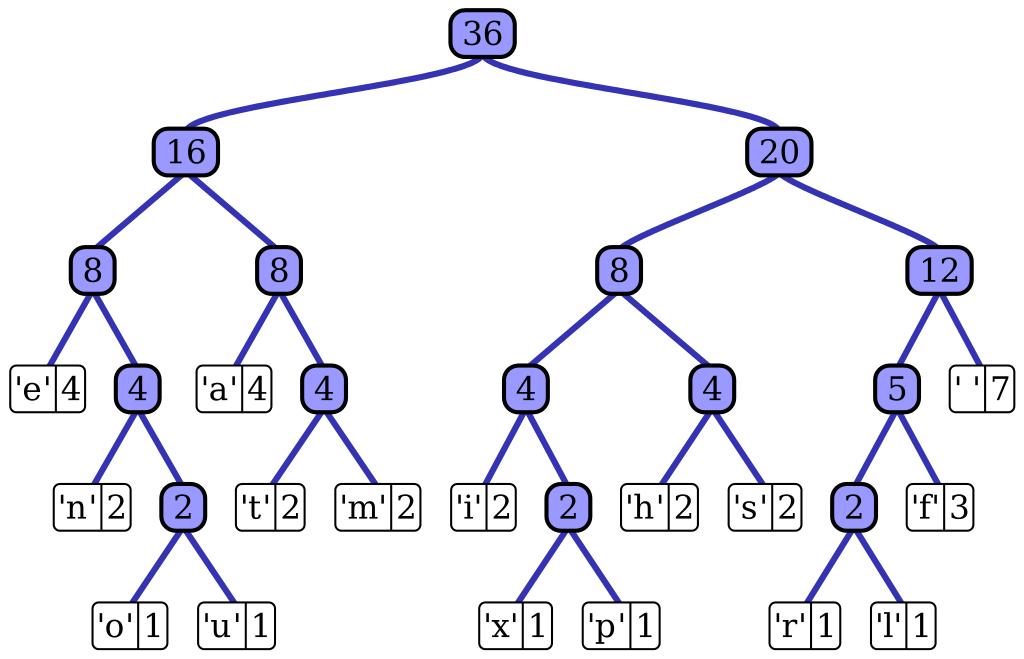
\includegraphics[width=0.7\textwidth]{huffman}
\end{figure}
In our alternative (and better way) we implement a queue with FIFO properties. The diagram above, taken from Wikipedia, shows what I call a `balanced Huffman tree'. Our objective for our `smart' tree is to generate a balanced tree which will allow us to have smaller codes for each character.

We first take our two smallest (i.e. lowest occurring) characters and merge them. We then put this to the queue.
We continue by taking the next smallest character and check if the value (i.e. frequency value) for this character is larger or equal to merged tuple we have stored in our queue. If such is the case, then we pop from the queue, merge the two and put the result back in the queue. If not, we allow the queue to remain unchanged while we draw another character and continue to merge the two characters we have at hand. We then put this back into the queue. We can continue this process until we have ran out of elements in our map but we ain't over yet.

We then use the \texttt{clean\_queue/1} method to merge elements without our queue. The smallest-first nature of our \texttt{min\_pop/1} method ensures that our queue is sorted from smallest to lowest `merged' value.

We pop two elements from our queue and merge them, putting the result back into the queue. We then take two more elements from our queue, merge and put back into the queue. We continue with this process until either the queue is empty or there is only element left in the queue. This final value is our Huffman tree.

\pagebreak
\begin{lstlisting}[language=Elixir, title=Smart way to generate the tree]
defmodule Praanto do
  def tree_start(map) do
    first([], map)
  end
  def first(fifo, map) do
    {kv1, map} = Mapper.min_pop(map)
    {kv2, map} = Mapper.min_pop(map)
    fifo = FIFO.push(fifo, merge(kv1, kv2))
    next(fifo, map)
  end
  def next(fifo, map) when map == %{} do
    clean_fifo(fifo)
  end
  def next(fifo, map) do
    {{k1, v1}, map} = Mapper.min_pop(map)
    {{:leaf, vx, lx, rx}, fifo} = FIFO.pop(fifo)
    case v1 >= vx do
      false ->
        fifo = FIFO.push_last(fifo, {:leaf, vx, lx, rx})
        map = Map.put(map, k1, v1)
        first(fifo, map)
      true ->
        fifo = FIFO.push(fifo, {:leaf, v1 + vx, {:node, k1}, {:leaf, vx, lx, rx}})
        next(fifo, map)
    end
  end
  def merge({k1, v1}, {k2, v2}) do
    {:leaf, v1 + v2, {:node, k1}, {:node, k2}}
  end
  def merge({k1, v1}, {:leaf, vx, lx, rx}) do
    {:leaf, v1 + vx, {:node, k1}, {:leaf, vx, lx, rx}}
  end
  def clean_fifo(fifo) do
    case FIFO.pop(fifo) do
      {last, []} ->
        last
      {{:leaf, v, l, r}, fifo} ->
        case FIFO.pop(fifo) do
          {{:leaf, v_last, l_l, r_l}, []} ->
            {:leaf, v + v_last, {:leaf, v, l, r}, {:leaf, v_last, l_l, r_l}}
          {{:leaf, v_last, l_l, r_l}, fifo} ->
            fifo =
              FIFO.push(fifo, {:leaf, v + v_last, {:leaf, v, l, r}, {:leaf, v_last, l_l, r_l}})
            clean_fifo(fifo)
        end
    end
  end
end
\end{lstlisting}